\section{Experiments}
\label{sec:experiments}

All test numbers in this section come from one logged read of the locked test sets (\cref{sec:data}); every
other number is on validation units. Intervals are 95\,\% cluster bootstraps over the split units (duplicate or
temporal groups, days for the ceilometer pairs), 1,000 resamples. Baselines are a linear probe on the best frozen
backbone of our own probe sweep (DINOv3 ViT-L/16 for in-domain genus, ViT-B/16 for cross-dataset \'etage) and a
ridge on the same frozen features for cloud-base height, so that every comparison isolates what the heads add.

\subsection{Pre-registered criteria}
\begin{table}[t]
\centering
\small
\begin{tabular}{llrlrll}
\toprule
 & Quantity & Val & Test [95\% CI] & Reference & Required & Holds \\
\midrule
C1 & LODO étage macro-F1, mean of the four folds & 0.548 & 0.540 & 0.529 & $\geq$ reference + 0.05 & no \\
C1 & in-domain genus macro-F1 (CCSN, MGCD) & 0.719 & 0.706 & 0.733 & $\geq$ reference $-$ 0.01 & no \\
C2 & Montenegro étage-set agreement / human ceiling & 1.047 & 0.926 & 0.900 & $\geq$ 0.90 & yes \\
C2 & Montenegro oktas $\pm$1 agreement / human ceiling & 1.027 & 0.963 & 0.900 & $\geq$ 0.90 & yes \\
C3 & CBH skill, OLDLR (CDLRA) pairs & 0.471 & 0.536 [0.440, 0.630] & 0.200 & $\geq$ 0.20 & yes \\
C3 & CBH skill, WESTE (CDLRB) pairs, OLDLR-only training & 0.448 & 0.436 [0.276, 0.585] & 0.100 & $\geq$ 0.10 & yes \\
C3 & CBH MAE (m), all pairs, against the frozen-feature ridge & 566 & 872 [679, 1055] & 1096 & $\leq$ 0.9 $\times$ reference & yes \\
C3 & 80 \% interval coverage with the P089 temperature and radius & 0.802 & 0.720 & 0.800 & 0.75–0.85 & no \\
\bottomrule
\end{tabular}
\caption{Pre-registered criteria on validation (Gate G4) and on the locked test sets, read once.}
\label{tab:criteria}
\end{table}

\Cref{tab:criteria} is the paper in one table. The three criteria were fixed before training with their
thresholds; two of the eight clauses fail on the test read and we leave them failed. C1 asked the heads to beat the
probe on cross-dataset \'etage by 0.05 macro-F1 and to match it within 0.01 on in-domain genus; the heads lead the
probe by \nLodoModel{} to \nLodoProbe{} (within the interval) and trail the larger ViT-L probe on genus
(\nIndGenusModel{} vs \nIndGenusProbe{}). C2 asked for 90\,\% of the expert ceiling on the five-rater set and holds
on both \'etage sets (\nCtwoEtage{}) and cover (\nCtwoOktas{}). C3 asked for skill over climatology at the seen site
and at a site never trained on, and for a 10\,\% MAE lead over the ridge; all three hold with the test intervals
clear of the thresholds. Its fourth clause, 80\,\% conformal coverage, does not: the intervals fitted on the spring
validation days cover \nCovEighty{} of the summer test pairs, where the climatology MAE itself grows from 1,147\,m
to \nMaeClim{}\,m. The calibration transfers worse than the point estimate.

\subsection{Recognition}
\begin{table*}[t]
\centering
\footnotesize
\begin{tabular}{llrr}
\toprule
Protocol & Source & STRATIA & Linear probe \\
\midrule
in-domain genus & CCSN & 0.591 [0.54, 0.63] & 0.549 [0.50, 0.59] \\
in-domain genus & MGCD & 0.821 [0.71, 1.00] & 0.918 [0.76, 0.95] \\
in-domain étage & ccsn & 0.719 [0.68, 0.76] & – \\
in-domain étage & mgcd & 1.000 [1.00, 1.00] & – \\
in-domain étage & montenegro & 0.680 [0.63, 0.72] & – \\
in-domain étage & almeria & 0.803 [0.68, 0.86] & – \\
LODO étage (held out) & ccsn & 0.451 [0.43, 0.47] & 0.396 [0.38, 0.41] \\
LODO étage (held out) & mgcd & 0.709 [0.62, 0.78] & 0.860 [0.79, 0.92] \\
LODO étage (held out) & montenegro & 0.367 [0.30, 0.45] & 0.463 [0.39, 0.53] \\
LODO étage (held out) & almeria & 0.634 [0.60, 0.66] & 0.397 [0.36, 0.43] \\
\bottomrule
\end{tabular}
\caption{Recognition on the locked test sets: STRATIA against the strongest linear probe of Stage F (ViT-L/16 for in-domain genus, ViT-B/16 for LODO étage), macro-F1 with cluster-bootstrap 95\% intervals.}
\label{tab:recognition}
\end{table*}

\Cref{tab:recognition} breaks the criteria down by source. The heads win where the probe has the least to go on
(CCSN genus with its alternatives, Almer\'ia and CCSN \'etage held out) and lose on MGCD, whose seven sky types a
linear probe already separates at 0.918, and on Montenegro held out, where the mid \'etage is rare (2\,\% of
images) and the heads over-predict ``high''. The error analysis (\cref{fig:confusion}) shows where the remaining
genus errors live: stratus and stratocumulus are swapped on 18.5\,\% of their CCSN rows, cirrus and cirrostratus
on 7.0\,\%, altostratus and nimbostratus on 6.4\,\%, and MGCD altocumulus is read as stratocumulus 71\,\% of the
time, pairs that human annotators also split on. The mid \'etage is the one the model misses most, on every source
that has it (35--46\,\% missed at the 0.5 threshold).

\begin{figure}[t]
\centering
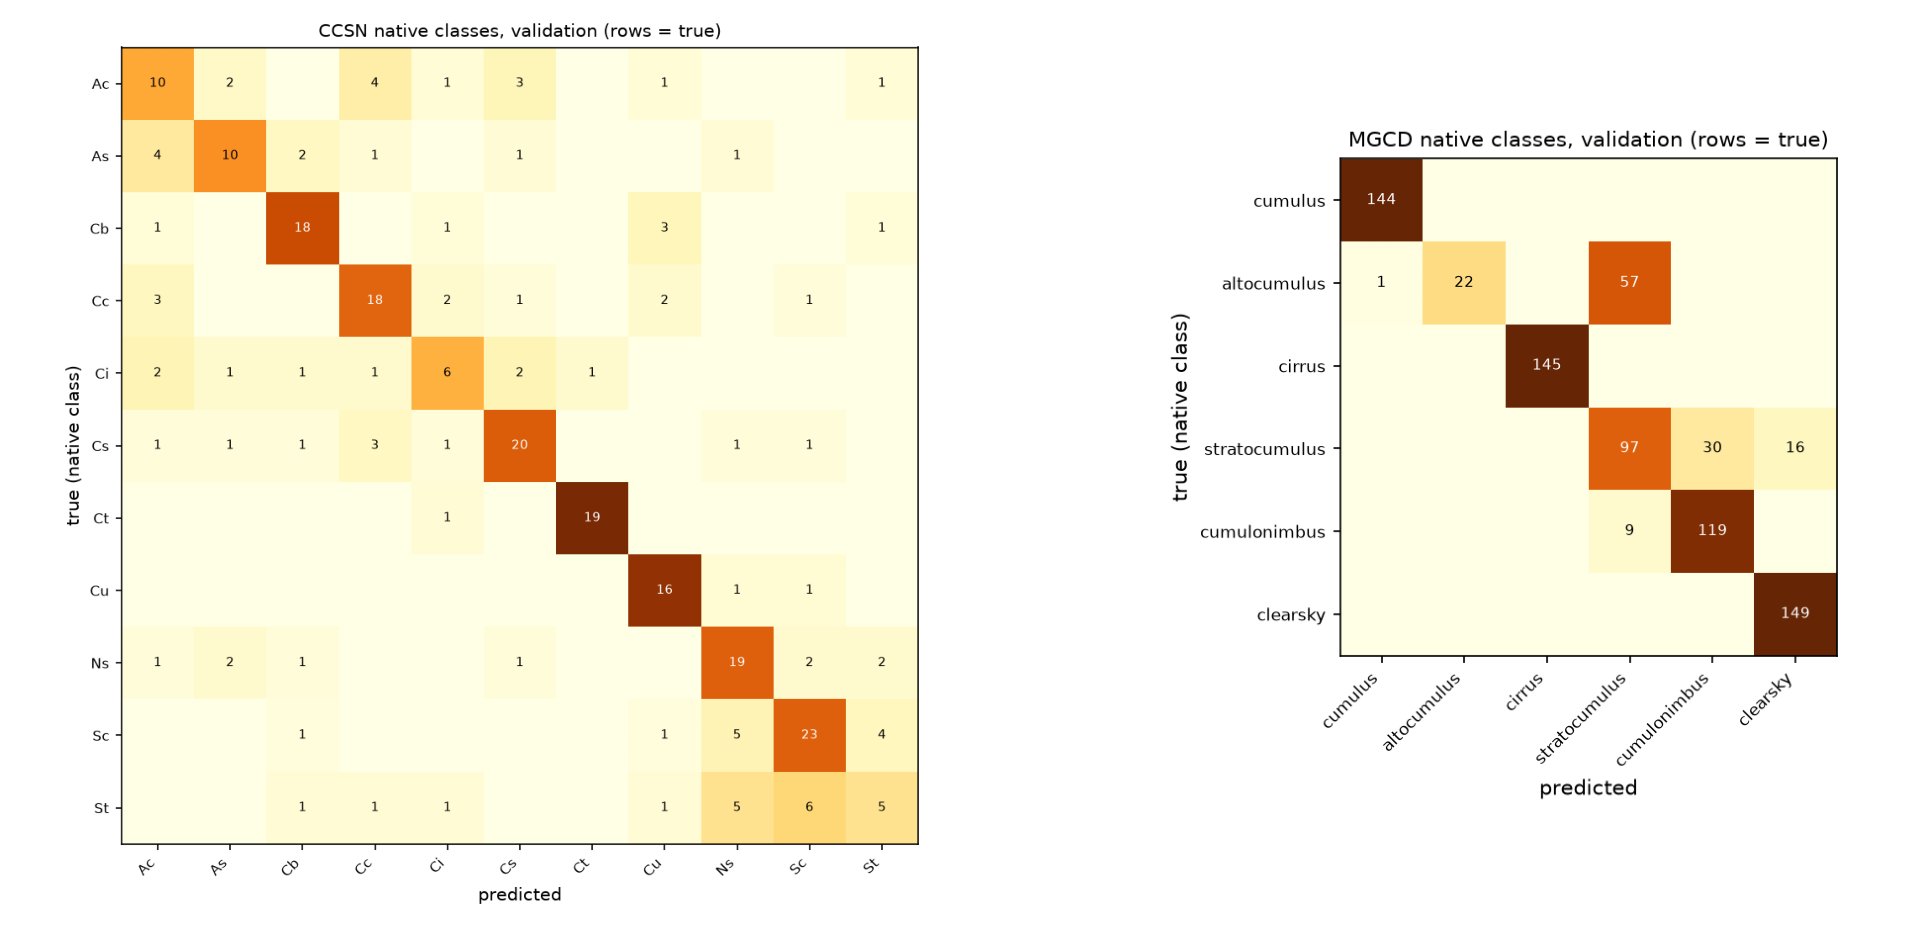
\includegraphics[width=\linewidth]{fig/genus_confusion.png}
\caption{Genus confusion on validation, native classes, for CCSN (left) and MGCD (right). Errors concentrate on
the pairs that the WMO hierarchy itself places as neighbours.}
\label{fig:confusion}
\end{figure}

\subsection{Against the expert ceiling}
\begin{table*}[t]
\centering
\footnotesize
\begin{tabular}{lrrrr}
\toprule
Quantity & Alpha (humans) & Alpha (+ model) & Model vs others & Human vs others \\
\midrule
étage set & 0.659 & 0.684 & 0.932 & 0.893 \\
oktas 0-8 & 0.960 & 0.956 & 0.892 & 0.909 \\
\bottomrule
\end{tabular}
\caption{STRATIA as a sixth Montenegro annotator (validation images): Krippendorff's alpha without and with the model, and agreement with the majority of the other raters.}
\label{tab:humanceiling}
\end{table*}

C2 compares with the ceiling as a ratio; \cref{tab:humanceiling} puts the model in the annotators' seats. Adding
STRATIA as a sixth rater raises Krippendorff's alpha on \'etage sets from \nAlphaEtageHumans{} to
\nAlphaEtageModel{} (the model agrees with the group more than the average human does) and leaves cover alpha
unchanged within 0.004. In leave-one-out terms the model agrees with the other raters' majority on
\nLooEtageModel{} of images against a human mean of \nLooEtageHumans{}, which ranks it second of six raters; on
cover it ranks last of six, at \nLooOktasModel{} against \nLooOktasHumans{}, close behind the humans. These are
validation images (the Montenegro test set is two blocks of days and too small to rank six raters).

\subsection{Cloud-base height}
\begin{table*}[t]
\centering
\footnotesize
\begin{tabular}{lrrrr}
\toprule
Model & MAE (m) [CI] & Skill [CI] & $\pm$500 m & 80\% cov. \\
\midrule
STRATIA (both sites in training) & 872 [679, 1055] & 0.566 [0.48, 0.66] & 0.546 & 0.720 \\
  OLDLR (CDLRA) & 933 [744, 1127] & 0.536 [0.44, 0.63] & 0.531 & 0.698 \\
  WESTE (CDLRB) & 813 [601, 1013] & 0.596 [0.50, 0.70] & 0.561 & 0.742 \\
STRATIA, geometry zeroed & 875 [680, 1050] & 0.565 [0.48, 0.66] & 0.546 & 0.764 \\
STRATIA trained on OLDLR only, tested on WESTE & 1134 [835, 1456] & 0.436 [0.28, 0.58] & 0.496 & 0.605 \\
Ridge on frozen features (P058) & 1096 [852, 1365] & 0.455 & 0.470 & – \\
Training climatology & 2012 & – & – & – \\
\bottomrule
\end{tabular}
\caption{Cloud-base height on the locked ceilometer-paired test pairs (2,965 cloudy frames, 25 days per site): MAE, skill over the training climatology, share within 500 m, and 80\% interval coverage with the validation-fitted calibration.}
\label{tab:cbh}
\end{table*}

\Cref{tab:cbh} reports the ceilometer-paired test pairs. The height head halves the climatology error and beats the
ridge on the same features by 20\,\% in MAE; trained on one station and tested on the other it keeps a skill of
\nSkillWeste{}, so what it learns is not a station's climatology. Zeroing the geometry at test time changes the
MAE by 3\,m, which says the head reads height from appearance, not from where the camera points (the SkyRay
ablations in \cref{tab:ablations} say the same for the global heads). Calibrated 95\,\% intervals cover
\nCovNinetyFive{} and the 80\,\% intervals \nCovEighty{}; \cref{fig:cbh} shows the per-pair scatter on the
validation days.

\begin{figure}[t]
\centering
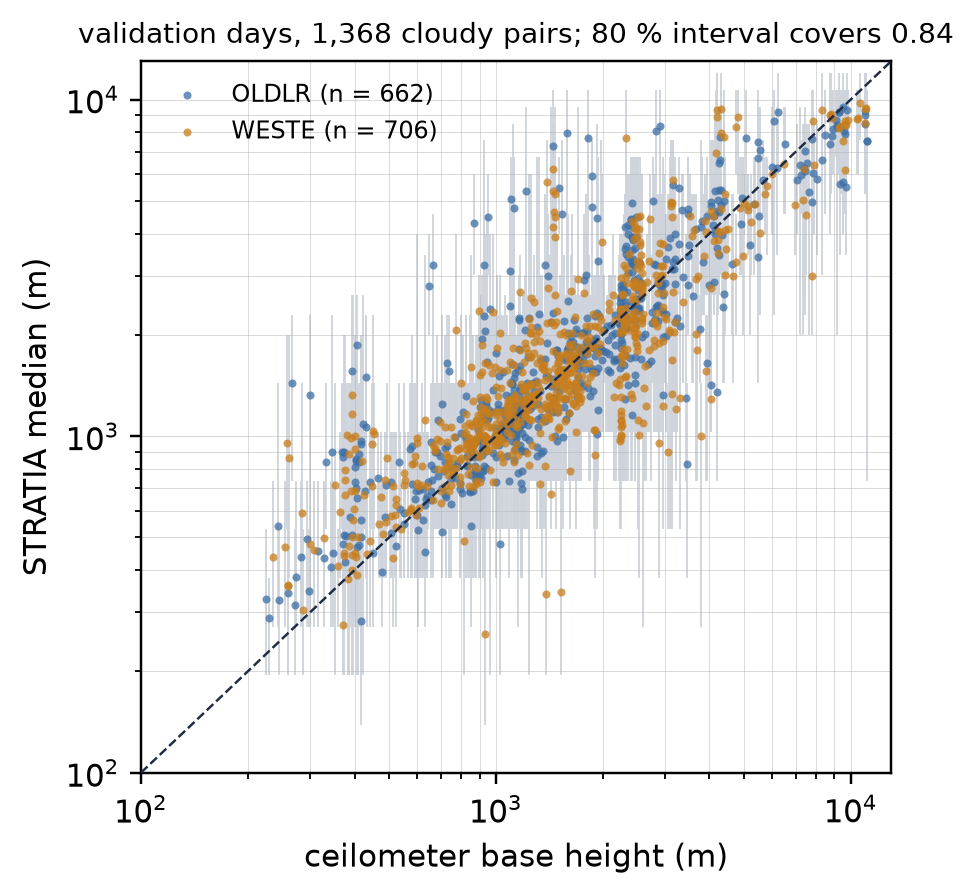
\includegraphics[width=\linewidth]{fig/cbh_scatter.png}
\caption{Predicted against ceilometer cloud-base height on the validation days (log axes), with the 80\,\%
conformal interval of each pair in grey.}
\label{fig:cbh}
\end{figure}

\subsection{Sky parse, OOD and glare}
The dense head reaches a sky/cloud/glare mIoU of \nSkyMiou{} on the pooled test masks and a layer mIoU of
\nLayerMiou{} on Almer\'ia; on the clear-sky test frames it still calls \nClearCloud{} of the pixels cloud, most of
it in the circumsolar region. The OOD score separates the owner's camera from the in-domain test frames at an
AUROC of \nOodAuroc{}. Under a synthetic Sun-glare corruption on validation, \'etage F1 drops from 0.838 to 0.760,
sky mIoU from 0.901 to 0.816, and the clear-sky cloud fraction rises from 0.29 to 0.47: glare is the single
failure mode we can name, and the parse rather than the recognition is what it breaks.

\subsection{Ablations}
\begin{table}[t]
\centering
\small
\begin{tabular}{llrr}
\toprule
Group & Variant & Étage F1 & Genus F1 \\
\midrule
reference & Gate G4 heads (geometry dropout 0.3, soft and set-valued targets, hier & 0.817 & 0.719 \\
geometry (SkyRay) & no geometry: ray map and Sun always dropped (p\_drop 1.0) & 0.809 & 0.720 \\
geometry (SkyRay) & geometry always given (p\_drop 0.0) & 0.829 & 0.709 \\
targets & hard targets: first listed genus, majority étages, majority okta & 0.794 & 0.729 \\
loss & no hierarchy loss (lambda\_h 0) & 0.813 & 0.712 \\
loss & uncertainty (Kendall) task weighting & 0.814 & 0.716 \\
Eye2Sky étage rows & without the ceilometer étage rows (indomain) & 0.823 & 0.738 \\
Eye2Sky étage rows (LODO) & held-out ccsn, with Eye2Sky étage rows & 0.489 & – \\
Eye2Sky étage rows (LODO) & held-out ccsn, without & 0.486 & – \\
Eye2Sky étage rows (LODO) & held-out mgcd, with Eye2Sky étage rows & 0.749 & – \\
Eye2Sky étage rows (LODO) & held-out mgcd, without & 0.871 & – \\
Eye2Sky étage rows (LODO) & held-out montenegro, with Eye2Sky étage rows & 0.360 & – \\
Eye2Sky étage rows (LODO) & held-out montenegro, without & 0.258 & – \\
Eye2Sky étage rows (LODO) & held-out almeria, with Eye2Sky étage rows & 0.593 & – \\
Eye2Sky étage rows (LODO) & held-out almeria, without & 0.327 & – \\
regularisation (P080) & head dropout 0 & 0.804 & 0.703 \\
regularisation (P080) & head dropout 0.3 & 0.817 & 0.743 \\
regularisation (P080) & weight decay 0 & 0.816 & 0.722 \\
regularisation (P080) & weight decay 0.2 & 0.815 & 0.715 \\
regularisation (P080) & no EMA & 0.820 & 0.711 \\
regularisation (P080) & EMA 0.999 & 0.812 & 0.708 \\
\bottomrule
\end{tabular}
\caption{Ablations of the global heads on validation data (one seed; the reference's three-seed spread is below 0.01): mean étage macro-F1 over the sources and mean genus macro-F1; the LODO rows give the held-out fold's étage F1.}
\label{tab:ablations}
\end{table}

\Cref{tab:ablations} varies the global heads one factor at a time on validation (one seed; the three reference
seeds spread by less than 0.01 in mean \'etage F1). Dropping the geometry always (\nAblNoGeo) or giving it always
(\nAblGeoAlways) brackets the reference (\nAblRef) within a point either way: SkyRay is cheap and does not hurt, but
on these sources the signal in the pixels dominates. Collapsing the set-valued and soft targets to one hard label
costs more (\nAblHard): the \emph{sets} are worth more than the geometry. Removing the hierarchy loss (\nAblNoH) and
uncertainty-weighting the tasks (\nAblKendall) are within noise of the reference. The weak \'etage rows derived
from the ceilometers are what make the all-sky folds transfer: without them the held-out Almer\'ia fold drops from
0.593 to 0.327 and Montenegro from 0.360 to 0.258, while MGCD, whose \'etages follow its seven sky types, gains;
the four-fold mean goes from 0.486 to the 0.548 of C1. Joint multi-task training and LoRA unfreezing of the last
blocks, tried in earlier stages, did not beat the staged cached-feature training that the released model uses
(layer mIoU 0.544 jointly against 0.559 staged); the released ablation tables report them.

\subsection{Efficiency}
\begin{table}[t]
\centering
\footnotesize
\begin{tabular}{lrr}
\toprule
Setting & Median ms & p95 ms \\
\midrule
PyTorch fp32, RTX 4050, batch 1 & 19.5 & 23.7 \\
PyTorch fp16, RTX 4050, batch 1 & 15.0 & 16.2 \\
PyTorch fp32, RTX 4050, batch 8 & 16.5 & 16.5 \\
ONNX Runtime CPU, batch 1 & 144.1 & 149.4 \\
desktop app, DirectML, RTX 4050, batch 1 & 29.2 & 33.0 \\
desktop app, ONNX Runtime CPU, batch 1 & 148.7 & 153.7 \\
Raspberry Pi 5 & – & – \\
\bottomrule
\end{tabular}
\caption{Latency per frame (median / p95 of repeated runs) of the deployed graph; 23.4 M parameters, 46 GFLOPs at 512 x 512.}
\label{tab:efficiency}
\end{table}

The exported graph has \nParamsM{}\,M parameters, of which \nHeadsParamsM{}\,M are above the frozen backbone, and
runs at \nGFlops{}\,GFLOPs for one 512$\times$512 frame (\cref{tab:efficiency}); inside the desktop application on a
laptop GPU through DirectML it takes \nLatencyDml{}\,ms per frame, and \nLatencyCpu{}\,ms on the CPU provider. The
Raspberry Pi 5 figure is left blank: the edge student is planned but not measured.

\subsection{A new camera from three afternoons}
\label{sec:b0268}
\begin{table}[t]
\centering
\small
\begin{tabular}{lrrrr}
\toprule
Model & Exact étage set & Oktas $\pm$1 & Top genus in set & OOD flagged \\
\midrule
zero-shot & 0.000 & 0.017 & 0.121 & 0.508 \\
adapted on three afternoons & 0.463 & 0.671 & 1.000 & 0.000 \\
rater vs rater (ceiling) & 0.911 & 0.771 & – & – \\
\bottomrule
\end{tabular}
\caption{The owner's camera (Arducam B0268), locked day 2026-10-20, 120 frames never used before the final evaluation; scored against each of the two annotators and averaged.}
\label{tab:b0268}
\end{table}

The released graph was pointed at the authors' own fisheye camera, a lens, exposure and horizon no training image
shares. Zero-shot (\cref{tab:b0268}) it is useless and says so: it agrees with the two annotators on
\nZsEtage{} of \'etage sets and \nZsOktas{} of cover within one okta on the locked fourth day, and flags \nZsOod{} of
the frames as out of distribution. Fine-tuning the global heads on the three earlier afternoons (273 frames, source
replay, regression guard) and re-exporting brings the agreement to \nAdEtage{} and \nAdOktas{}, with the top genus
inside the annotators' set on every frame and no frame flagged; the two annotators agree with each other on
0.911 and 0.771. The adapted graph is the one the application ships, and the fourth day was read once, after the
graph was frozen.
